\section{Wie sieht ein Data Lake aus}

\begin{figure}
  \begin{center}
    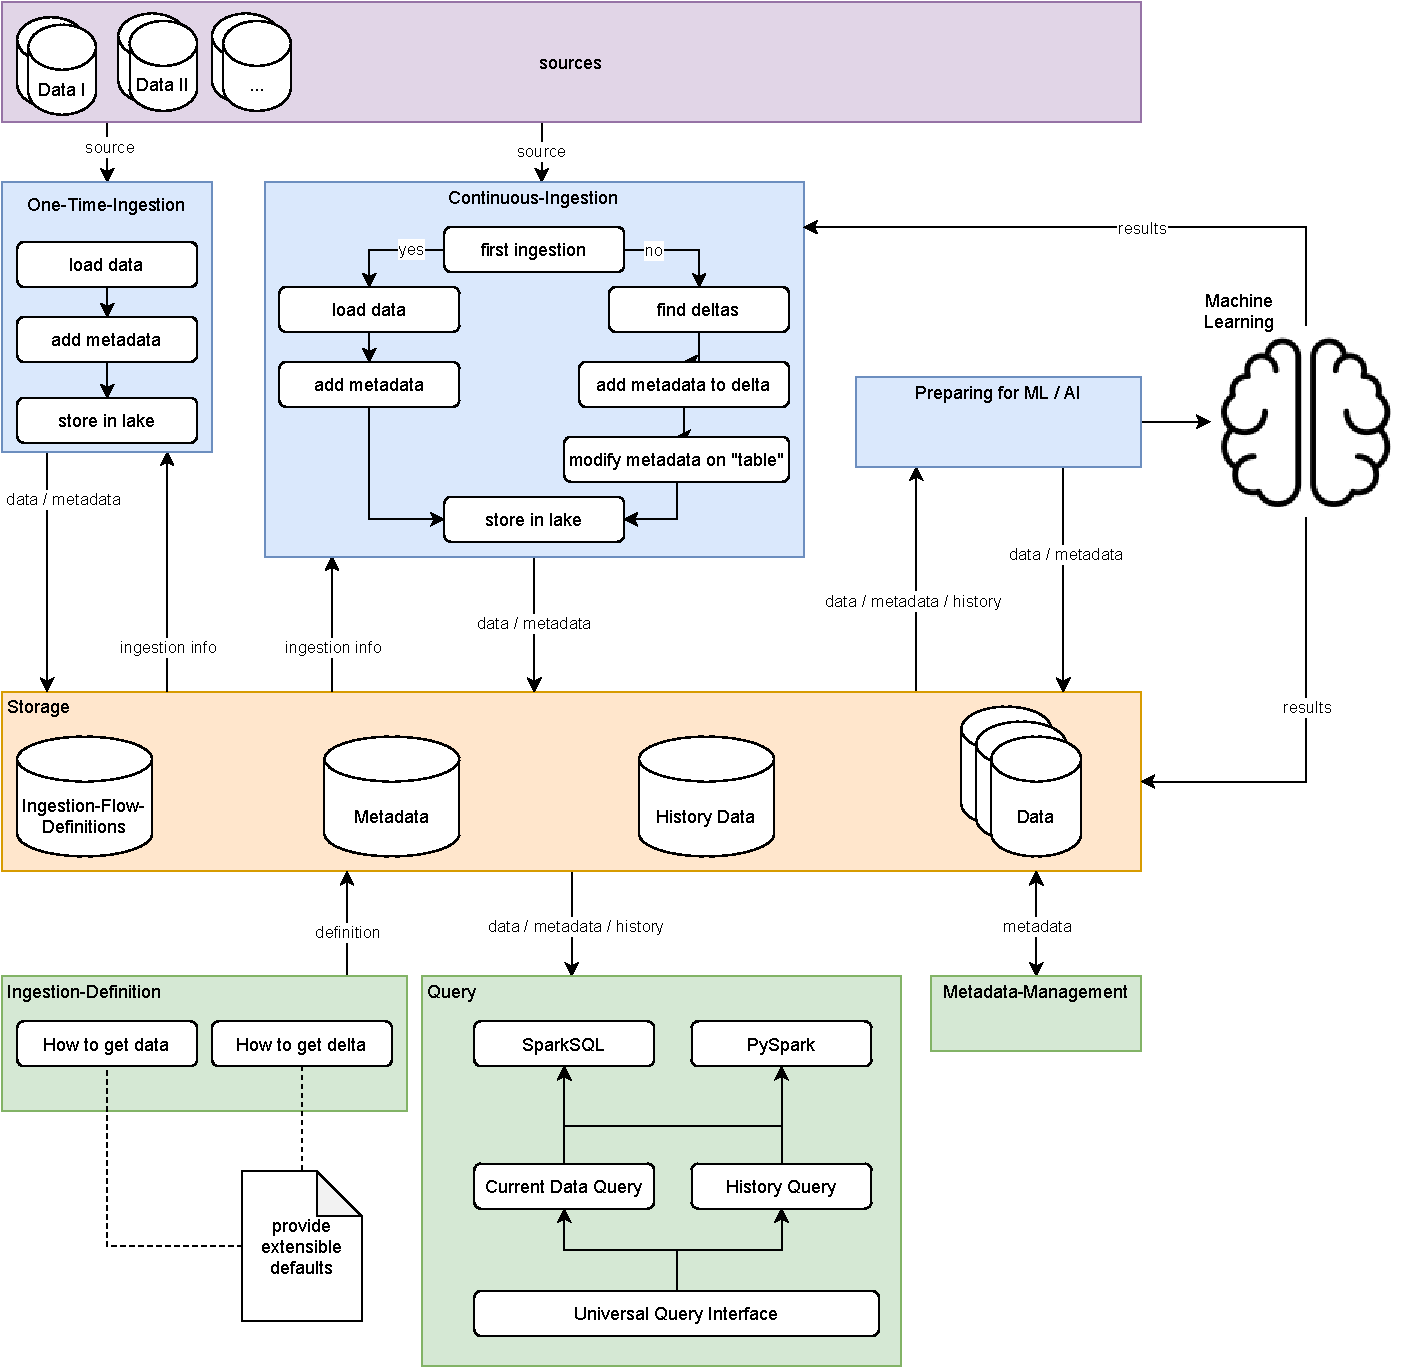
\includegraphics[width=\textwidth]{Grafiken/arch.pdf}
    \caption{Architektur einse Data-Lake-Systems}
    \label{fig:dl-arch}
  \end{center}
\end{figure}
In \fref{fig:dl-arch} wird ein Data-Lake-System dargestellt, das alle in der Einleitung angesprochenen Punkte berücksichtigt.
Hier ist nochmal zu sehen, dass Daten sowohl über eine einmalige als auch eine kontinuierliche Ingestion in den Data Lake gelangen können.
Dabei verwenden beide Komponenten eine einheitliche und allgemeine Definition (Ingestion-Flow-Definition) über die von einer einfachen Datenbank als Quelle bis hin zu einem komplexen Ablauf von Abfragen gegen eine API festgelegt werden können.
Das Ziel ist es, die Ingestion-Schnittstelle komplett unabhängig von der Datenquelle zu machen.
In der Continuous-Integration ist zusätzlich zu sehen, dass hier neben dem reinen Laden der Daten auch das Finden und Speichern von Deltas eine Rolle spielt, da hier durch das kontinuierliche Laden der Daten Änderungen in den Daten anfallen.

Die Daten des Data-Lake-Systems können dann für Machine-Learning aufbereitet und verwendet werden.
Ergebnisse des Machine-Learnings werden wieder im Data Lake gespeichert.
Die Herausforderung dabei ist, die Ergebnisse mit in den Versionsverlauf einzupflegen.
Eine Möglichkeit wäre das Machine-Learning als Datenquelle an die Ingestion mit anzubinden.
Um diese Schwierigkeit zu umgehen, kann man die Informationen auch direkt in den Data Lake zurückschreiben.
Dabei verliert man aber alle Vorteile des Versionsverlauf.

Für die Benutzer des Data-Lake-Systems stehen drei Interaktionspunkte zur Verfügung.
Der erste ist die Erstellung und Bearbeitung von Ingestion-Definitions.
Diese beschreiben, wie Daten aus verschiedenen Quellen geladen werden sollen und wie man in den Datenquellen Änderungen findet.
Um das System benutzerfreundlicher zu gestalten, sollten bereits Definitionen für gängige Systeme vorhanden sein, die dann erweitert oder als Vorlage genutzt werden können.
Als zweites steht eine Abfragen-Schnittstelle zur Verfügung, die einen einheitlichen Zugriff auf die verschieden Abfragemöglichkeiten des Systems stellt.
Zum Schluss gibt es noch die Metadatenverwaltung, bei der zu den automatisch erstellten Metadaten weitere hinzugefügt werden können.